~\\
~\\
\subsection{Pockels-Effekt/ Linearer elektrooptischer Effekt}
Der Pockels-Effekt ist auf der Tatsache begründet, dass die Permittivität $\epsilon=\frac{\partial D}{\partial E}$ nicht konstant ist, sondern vom elektrischen Feld abhängt. Das bedeutet, dass D nicht rein linear von E abhängt, sodass gilt: $\epsilon=a+2bE+3cE^{2}+...$. Da der Brechungsindex von der Permittivität abhängt, bedeuten Anderungen in $\epsilon$ auch Anderungen in diesem. Andert sich der Brechungsindex eines Kristalls durch ein äußeres elektrisches Feld, so spricht man vom elektrooptischen Effekt. Der lineare Anteil in der Formel $2bE$ bewirkt den Pockels-Effekt.\\
\begin{floatingfigure}[l]{11cm}
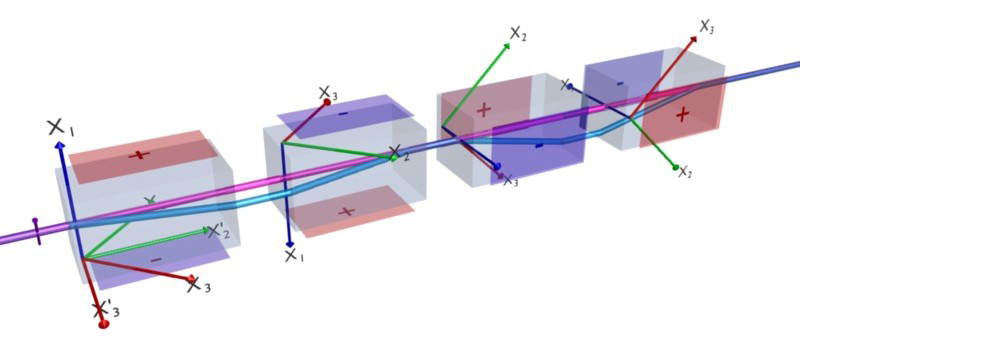
\includegraphics[scale=0.4]{aufbaupock.png}
\caption{Pockels-Zelle; Quelle: [ver]}
\end{floatingfigure}
Um kleine Veränderungen von $\epsilon$ und somit im Brechungsindex n messen zu können, kann die Doppelbrechung ausgenutzt werden. Andert sich der Brechnungsindex, so wird der Indexellipsoid umgeformt. In diesem Versuch werden Kristalle verwendet, in welchen nur der lineare elektrooptische Effekt, also der Pockels-Effekt, von Bedeutung ist. Diese sind in einem $45\,^{\circ}-Y-Cut$ (s. [Ver]) angeordnet. Mit dem Versuch messen wir die Halbwellenspannung $U_{\lambda/2}$: Für eine "Pockels-Zelle" ist das diejenige Spannung, die eine Phasenverschiebung von $\pi$ induziert.\\

Die Pockels-Zelle, welche wir verwenden, ist aus vier Kristallen aufgebaut. Die Anzahl ist wegen der Doppelbrechung so festgesetzt: Die zwei Kristallpaare bestehen aus jeweils zwei Kristallen derselben Orientierung. Die Paare sind zueinander um $90\,^{\circ}$ verschoben. Dieser Aufbau bewirkt folgendes: Das eintreffende Licht erreicht den ersten Kristall und wird aufgespalten. Der nächste Kristall macht diese Aufspaltung rückgängig. Um die natürliche Phasenverschiebung auszugleichen (damit nur die durch den Pockels-Effekt verursachte Verschiebung übrig bleibt), wird das zweite Kristallpaar gebraucht: Der dritte Kristall hat nämlich eine um $90\,^{\circ}$ verschobene Orientierung. Da das Licht aber wieder aufgespalten wird, benötigt man den 4. Kristall, um diesen Effekt rückgängig zu machen.